
% This work is licensed under the Creative Commons Attribution-Noncommercial-Share Alike 3.0 New Zealand License.
% To view a copy of this license, visit http://creativecommons.org/licenses/by-nc-sa/3.0/nz
% or send a letter to Creative Commons, 171 Second Street, Suite 300, San Francisco, California, 94105, USA.

\documentclass[12pt,leqno,a4paper]{book}
\usepackage[dvips]{graphicx}
\usepackage[usenames]{color}
\usepackage[colorlinks,pdfauthor={Jason R Briggs},pdftitle={Snake Wrangling for Kids - Learning to Program with Python},pdfsubject={Programming for Kids},pdfkeywords={python,kids,programming}]{hyperref}
\usepackage{longdiv}
\usepackage{makeidx}
\usepackage{versions}
\usepackage[absolute]{textpos}
\usepackage{wrapfig}
\usepackage{eso-pic}

\parindent 1cm
\parskip 0.2cm
\topmargin 0.2cm
\oddsidemargin 1cm
\evensidemargin 0.5cm
\textwidth 15cm
\textheight 21cm

\definecolor{PaleBlue}{rgb}{0.95,0.95,1}

\newenvironment{listing}
{\begin{list}{}{\setlength{\leftmargin}{1em}}\item\footnotesize\samepage}
{\end{list}}

\newenvironment{listingignore}
{\begin{list}{}{\setlength{\leftmargin}{1em}}\item\footnotesize\samepage}
{\end{list}}

\newcommand{\code}{\textcolor{OliveGreen}\bfseries}

\includeversion{FRONTCOVER}
\excludeversion{WINDOWS}
\excludeversion{MAC}
\includeversion{LINUX}

\title{Snake Wrangling for Kids - Learning to Program with Python}
\author{Jason R Briggs}

\makeindex

\begin{document}

\pagestyle{empty}
\frontmatter
\begin{FRONTCOVER}
\begin{titlepage}
\begin{textblock*}{210mm}(0mm,0mm)
   
\includegraphics[width=0.9\paperwidth]{cover-ru.eps}
\end{textblock*}
\begin{flushright}
\begin{WINDOWS}

\includegraphics[width=40mm]{windows-edition.eps} 
\end{WINDOWS}
\begin{MAC}

\includegraphics[width=40mm]{mac-edition.eps} 
\end{MAC}
\begin{LINUX}

\includegraphics[width=40mm]{linux-edition.eps} 
\end{LINUX}
\end{flushright}
\end{titlepage}
\end{FRONTCOVER}

\noindent
\textsf{\emph{Укрощение Змей Для Детей - Учимся Программировать с Python}}\\
Автор Джейсон Р. Бриггс\\
\\
Version 0.7.7
\\\\
Copyright \copyright 2007.\\
\\
Cover art and illustrations by Nuthapitol C.\\
\\
\noindent
\textsf{\emph{This book has been completely rewritten and updated, with new chapters (including developing graphical games), and new code examples. It also includes lots of fun programming puzzles to help cement the learning. Published by No Starch Press - available here: \href{http://nostarch.com/pythonforkids}{Python for Kids}. Also find more info \href{http://jasonrbriggs.com/python-for-kids/}{here}.}}
\\
\\
\linebreak
\noindent
Website:\\ \href{http://www.briggs.net.nz/log/writing/snake-wrangling-for-kids}{http://www.briggs.net.nz/log/writing/snake-wrangling-for-kids}\\ 
\\
\noindent
Thanks To:\\
Guido van Rossum (for benevelont dictatorship of the Python language), the members of the \href{http://www.python.org/community/sigs/current/edu-sig/}{Edu-Sig} mailing list (for helpful advice and commentary), author \href{http://www.davidbrin.com/}{David Brin} (the original \href{http://www.salon.com/tech/feature/2006/09/14/basic/}{instigator} of this book), Michel Weinachter (for providing better quality versions of the illustrations), and various people for providing feedback and errata, including: Paulo J. S. Silva, Tom Pohl, Janet Lathan, Martin Schimmels, and Mike Cariaso (among others).  Anyone left off this list, who shouldn't have been, is entirely due to premature senility on the part of the author.\\

\noindent
License:\\
\\

\includegraphics[width=40mm]{by-nc-sa.eps}\\
This work is licensed under the Creative Commons Attribution-Noncommercial-Share Alike 3.0 New Zealand License. To view a copy of this license, visit\\ \href{http://creativecommons.org/licenses/by-nc-sa/3.0/nz/}{http://creativecommons.org/licenses/by-nc-sa/3.0/nz/} or send a letter to Creative Commons, 171 Second Street, Suite 300, San Francisco, California, 94105, USA.\\

\noindent
Below is a summary of the license.\\

\noindent
You are free:
\begin{itemize}
 \item \textbf{to Share} — to copy, distribute and transmit the work 
 \item \textbf{to Remix} — to adapt the work
\end{itemize}
\noindent
Under the following conditions:
\begin{description}
 \item[Attribution.] You must attribute the work in the manner specified by the author or licensor (but not in any way that suggests that they endorse you or your use of the work).
 \item[Noncommercial.] You may not use this work for commercial purposes.
 \item[Share Alike.] If you alter, transform, or build upon this work, you may distribute the resulting work only under the same or similar license to this one.
\end{description}

\noindent
For any reuse or distribution, you must make clear to others the license terms of this work.\\

\noindent
Any of the above conditions can be waived if you get permission from the copyright holder.\\

\noindent
Nothing in this license impairs or restricts the author's moral rights.\\

\vspace*{4cm}
\begin{center}

\includegraphics[width=5cm]{python-powered.eps}
\end{center}

\mainmatter

\pagestyle{plain}

\pagenumbering{roman}
\tableofcontents

\include{preface}

\pagestyle{headings}
\pagenumbering{arabic}

% ch1.tex
% This work is licensed under the Creative Commons Attribution-Noncommercial-Share Alike 3.0 New Zealand License.
% To view a copy of this license, visit http://creativecommons.org/licenses/by-nc-sa/3.0/nz
% or send a letter to Creative Commons, 171 Second Street, Suite 300, San Francisco, California, 94105, USA.


\chapter{Не все змеи кусаются}\label{ch:notallsnakeswillsquishyou}

Скорее всего, ты получил эту книгу на день рождения. Или, возможно, на Новый Год. Тётя Надя собиралась подарить тебе два разных носка огромного размера (которые ты не захотел бы носить даже, когда вырастешь). Вместо этого, она услышала чей-то разговор о книжке, которую можно напечатать, и вспомнив, что у тебя был один из этих компьютеров, которым ты пытался научить её пользоваться в прошлый Новый Год (ты сдался, когда она стала пытаться разговаривать с мышкой), попросила распечатать ей ещё одну копию книги. Просто будь благодарен, что не получил те замшелые старые носки.

Я надеюсь, ты не слишком разочарован тем, что это я выскочила из подарочной упаковки, вместо тех носков. Не слишком уж разговорчивая (ладно, совсем не разговаривающая) книга, со зловещего вида названием на обложке про ``Изучение $\ldots$''.
Но задумайся на минутку о моих чувствах. Если бы ты был героем одного из романов про волшебников, что стоят в твоем книжном шкафу, у меня, вероятно, были бы зубы... или даже глаза. У меня внутри были бы движущиеся картинки, или я бы издавала всякие стонущие и завывающие звуки, когда ты перелистываешь мои страницы. Вместо этого я распечатана на листах обычной бумаги формата А4 с помятыми уголками, сшитых степлером или засунутых в папку. Хотя, откуда бы мне знать---у меня же нет глаз.
\\
\\
\emph{Эх, я бы все отдала за комплект хороших, острых зубов$\ldots$}
\\
\\
Однако, всё не так плохо, как кажется. Хоть я и не могу говорить ... или кусать за пальцы, когда ты отворачиваешься... Я могу рассказать тебе немного о том, что заставляет компьютеры работать. Не физически, благодаря проводам, микросхемам, кабелям и устройствам, которые, наверняка, ударят тебя током, если ты прикоснёшься к ним (поэтому, не трогай!!)---а про скрытые штуки, те, что работают внутри всех этих проводов, микросхем и кабелей и делают компьютеры по настоящему полезными.

\begin{wrapfigure}{r}{0.5\textwidth}
\begin{center}

\includegraphics[width=0.48\textwidth]{electrocute.eps}
\end{center}
\end{wrapfigure}

Это немного похоже на мысли, бегающие внутри твоей головы. Если бы у тебя не было мыслей, ты бы сидел на полу своей спальни, рассеяно глядя на дверь, и пускал слюни на свою футболку. Без \emph{программ}, компьютеры были бы полезны только в качестве подставки для ног---и даже тогда они были бы не слишком полезны, потому что ты бы постоянно спотыкался об них по ночам. Ведь нет ничего хуже, чем удариться ногой в темноте.
\\
\\
\emph{Я всего лишь книга, но даже я знаю это. }
\\
\\
У твоей семьи может быть Playstation, Xbox или Wii, стоящий в гостиной - они не используются без программ(игр) которые для них сделали. Ваш DVD-плеер, возможно, ваш холодильник и даже ваша машина - всё имеет компьютерные программы, которые делают эти вещи более полезными, чем они были бы без таких программ. Ваш DVD-плеер имеет программу позволяющую проиграть изображение записанное на DVD; ваш холодильник имеет программу, контролирующую потребление электричества, но позволяющую оставаться еде холодной; ваша машина возможно имеет компьютер, который предупреждает водителя об опасности.\\
Если вы знаете, как писать компьютерные программы, вы можете делать разные полезные штуки. Возможно, писать свои собственные игры. Создавать web страницы, которые действительно делают что-то полезное, а не просто красиво смотрятся. Умение программировать, возможно, даже поможет тебе с домашними заданиями.\\
\\
Как бы то ни было, пора переходить к чему-то более интересному.

\section{Несколько Слов О Языке}

Точно также, как у людей, наверняка, у китов, возможно, у дельфинов и может быть даже у родителей (хотя это спорно), у компьютеров тоже есть собственный язык. На самом деле, как и у людей, у них больше одного языка. Есть языки, охватывающие почти все буквы алфавита. A, B, C, D и E - это не только буквы английского алфавита, это ещё и языки программирования (которые доказывают, что у взрослых нет воображения, и им следовало бы почитать словарь или тезаурус прежде, чем давать чему-то название).

Есть языки программирования, названные в честь людей, названные с помощью простых сокращений (по заглавным буквам нескольких слов), и ещё несколько, названных в честь телешоу. О, и если ты добавишь несколько плюсов и решёток (+, \#) после пары тех букв, что я перечислил---это будет ещё несколько языков программирования. И что еще хуже, некоторые из языков почти одинаковые, и лишь слегка различаются.
\\
\\
\emph{Что я тебе говорил? Никакого воображения! }
\\
\\
К счастью, многие из этих языков вышли из употребления, или полностью исчезли; но список различных способов "поговорить" с компьютером по-прежнему до неприятного велик. Я собираюсь обсудить только один из них---в противном случае мы не смогли бы даже начать.
\\
Было бы более продуктивно сидеть в твоей спальне и пускать слюни на футболку$\ldots$

\section{Семейство Неядовитых\textbackslashСдавливающих Змеев$\ldots$}

$\ldots$или, для краткости, Питоны.

Помимо того, что Питон (англ. Python)\index{Python} это змея, это еще и язык программирования. Однако, он не был назван в честь безногой рептилии; скорее, это один из немногих языков программирования по имени телешоу. Монти Пайтон (Monty Python) было популярным в 1970-х годах британским комедийным шоу (которое, на самом деле остается популярным и по сей день), но ты должен быть определенного возраста, чтобы считать его забавным. Любой в возрасте до$\ldots$, скажем, 12$\ldots$ удивился бы, почему это кому-то нравится\footnote{Кроме танца хлопающей рыбы. Это смешно, независимо от того, сколько вам лет}.

У Питона (который язык программирования, а не змея или телешоу) есть ряд особенностей, которые делают его чрезвычайно полезным при изучении программирования. В нашем случае, сейчас, самая важная причина в том, что ты можешь запустить его и начать что-то делать по настоящему быстро.

Это та самая часть, где ты надеешься, что мама, папа (или кто у вас отвечает за компьютер), прочитал специальную часть в начале книги с надписью ``Примечание для мам и пап''.

\noindent
Есть хороший способ узнать, действительно ли они прочитали её:

\begin{WINDOWS}
Нажми кнопку с окошком \includegraphics*[width=12mm]{win-home.eps} внизу слева экрана, начни печатать 'command line' и справа в строке поиска должна появиться программа 'Python (command line)'. Нажми на `Python (command line)' и ты должен увидеть что-то похожее на картинку~\ref{fig2}.

\begin{figure}
\begin{center}

\includegraphics[width=80mm]{figure1.eps}
\end{center}
\caption{Python в меню Windows.}\label{fig1}
\end{figure}

\begin{figure}
\begin{center}
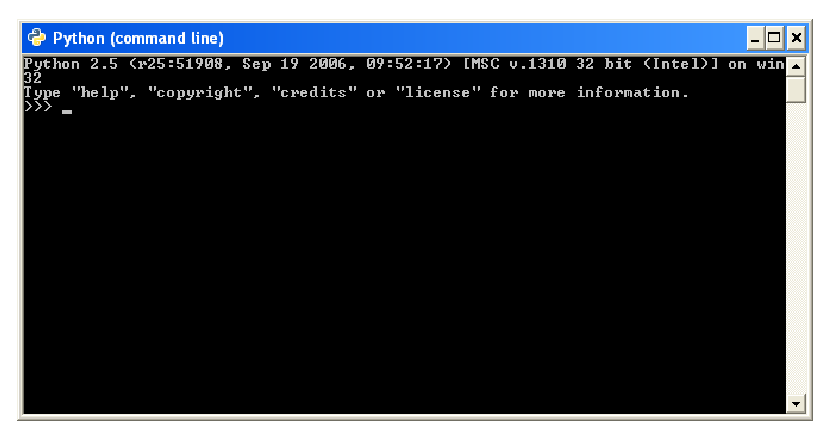
\includegraphics[width=135mm]{figure2.eps}
\end{center}
\caption{Консоль Python в Windows.}\label{fig2}
\end{figure}
\end{WINDOWS}

\begin{MAC}
В Finder, слева ты должен видеть раздел `Applications'.  Нажми на него, и затем найди программу под названием `Terminal' (она вероятно будет в папке с названием`Utilities').
Нажми на `Terminal' и, когда он запустится, введи 'python' и нажми клавишу 'enter'.  Ты должен теперь смотреть на окно, которое выглядит как на рисунке~\ref{fig3}.

\begin{figure}
\begin{center}
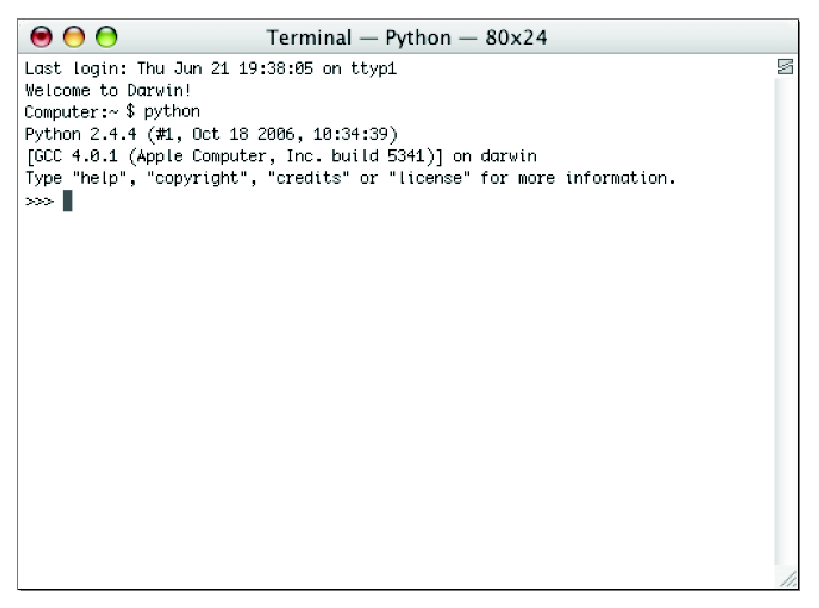
\includegraphics[width=85mm]{figure3.eps}
\end{center}
\caption{Консоль Python в Mac OSX.}\label{fig3}
\end{figure}
\end{MAC}

\begin{LINUX}
Спроси маму или папу, какую именно программу терминала тебе следует использовать (он может называться одной из этих: `Konsole', `rxvt', `xterm' или любая другая из десятка других---поэтому тебе скорее всего нужно спросить).  Запусти программу терминала и напечатай `python' (без кавычек), и нажми enter.  Ты должен увидеть что-то похожее на картинку~\ref{fig4}.

\begin{figure}
\begin{center}
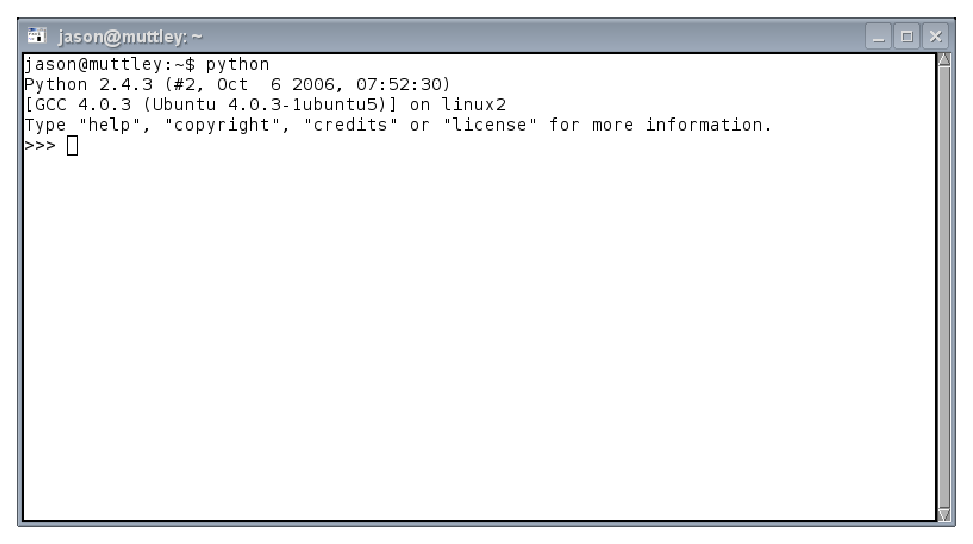
\includegraphics[width=80mm]{figure4.eps}
\end{center}
\caption{Консоль Python в Linux.}\label{fig4}
\end{figure}
\end{LINUX}

\subsection*{\color{BrickRed}Если ты обнаружил, что они не прочитали раздел в начале книги$\ldots$}

$\ldots$потому что чего-то не хватает, когда ты пытаешься следовать этим инструкциям---тогда отлистай в начало книги, подсунь её им под нос пока они читают свои книжки, и с надеждой повторяй ``пожалуйста пожалуйста пожалуйста пожалуйста'', снова и снова, пока это не начнёт надоедать, это должно сработать, если у тебя возникают сложности убедить их встать с дивана.  Конечно, кроме этого, ты можешь сам открыть начало книги и самостоятельно выполнить указанные там инструкции, чтобы установить Python.

\section{Твоя первая программа на Python}

Надеюсь, если ты дочитал до это места, у тебя уже получилось запустить консоль Python, которая позволяет выполнять программы и команды языка Python. Когда ты впервые запустишь эту консоль (или после того, как наберешь в ней первую команду), ты увидишь то, что называется `приглашение' (англ. prompt).  В консоли Python \index{Python console} приглашение выглядит в виде трёх треугольников или знаков больше ($>$), указывающих вправо:

\begin{listing}
\begin{verbatim}
>>>
\end{verbatim}
\end{listing}
Если ты составишь достаточное количество команд Python вместе, у тебя получится программа, которую ты сможешь запускать не только в консоли$\ldots$ но мы пока не станем усложнять, а будем вводить команды прямо в консоли, после приглашения ($>>>$). Так почему бы уже не начать, напечатав следующую команду (если нужно, спроси у родителей, как переключать ввод между русским и английским):

\begin{listing}
\begin{verbatim}
print("Привет Мир")
\end{verbatim}
\end{listing}

Убедись, что ты добавил кавычки (вот эти: $"$ $"$) и нажал ввод (Enter) в конце строки. Скорее всего ты увидишь что-то подобное:

\begin{listing}
\begin{verbatim}
>>> print("Привет Мир")
Привет Мир
\end{verbatim}
\end{listing}

Снова появится приглашение, давая тебе понять, что консоль Python готова принимать новые команды.

\noindent
Поздравляю! Ты только что создал свою первую программу на языке Python.  \code{print} это функция, которая выводит в консоль всё, что находится у неё между скобок--мы ещё не раз будем её использовать.

\section{Твоя вторая программа на Python$\ldots$опять тоже самое?}

Программы Python не были бы так полезны если бы тебе приходилось печатать её команды каждый раз, когда ты хотел бы что-то сделать---или если бы ты написал команду для кого-нибудь, и ему пришлось бы напечатать её перед тем, как начать использовать.

Текстовый редактор, который ты, возможно, используешь для своих школьных заданий, содержит, где-то от 10 до 100 миллионов строк кода. В зависимости от того, как много строк ты напечатаешь на одном листе (и будешь ли печатать с двух сторон или с одной), получилось бы 400,000 страниц$\ldots$ или стопка бумаги 40 метров высотой.
Просто представь, чтобы отвезти эту программу из магазина домой, потребовалось бы несколько ходок до машины, чтобы перенести так много бумаги$\ldots$

$\ldots$и тебе лучше надеятся, чтобы не было сильного ветра, пока ты носишь эти стопки бумаги. К счастью, есть альтернативный способ всему этому печатанию---иначе никто ничего не смог бы сделать.

\begin{center}
\includegraphics*[width=85mm]{pullinghair.eps}
\end{center}

\begin{WINDOWS}
Открой Блокнот (нажми на окошко внизу слева и начни печатать ``блокнот'', а потом нажми мышкой на найденную программу Блокнот), и напечатай команду print точно так же, как ты её печатал до этого в консоли:

\begin{listing}
\begin{verbatim}
print("Привет Мир")
\end{verbatim}
\end{listing}
Нажми на меню Файл (в Блокноте), затем Сохранить, и, когда попросят ввести имя файла, назови его \emph{hello.py} и сохрани его на Рабочем столе.  Дважды кликни на иконку с именем hello.py на Рабочем столе (смотри рисунок~\ref{fig5}) и ты увидишь, как на мгновение появится консоль Windows.  Она исчезнет слишко быстро, чтобы что-то заметить, но в консоли будут напечатаны слова ``Привет Мир''---мы вернемся к этому примеру позднее и докажем, что они там появляются.\\

\begin{figure}
\begin{center}
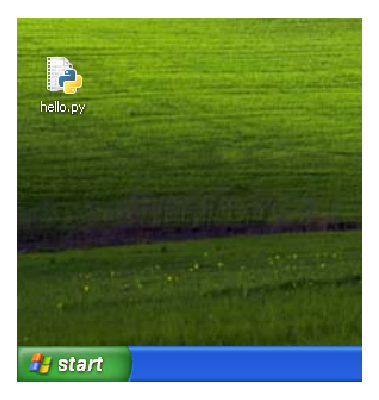
\includegraphics{figure5.eps}
\end{center}
\caption{Иконка hello.py на Рабочем столе Windows.}\label{fig5}
\end{figure}
\end{WINDOWS}

\begin{MAC}
Open up the Text Editor by clicking on its icon.  It may be in the Dock at the bottom of the screen \includegraphics*[width=12mm]{textedit-icon.eps}, or look for this icon \includegraphics*[width=19mm]{textedit-icon2.eps} in the Applications list in Finder.  Type the print command exactly as you typed it into the console earlier:

\begin{listing}
\begin{verbatim}
print("Hello World")
\end{verbatim}
\end{listing}

Click on the File menu, then click on Save, and when you are prompted for a file name, call it hello.py and save it into your home directory (your home directory is on the left under Places--ask Mum or Dad to point it out for you).

Open the `Terminal' application again--it will automatically start up in your home directory--and type the following:

\begin{listing}
\begin{verbatim}
python hello.py
\end{verbatim}
\end{listing}

You should see Hello World written to the window exactly as it was when you typed the command in the Python console.

\end{MAC}

\begin{LINUX}
Open a text editor (again you might have to ask Mum or Dad which one to use), then type the print command exactly as you typed it into the console:

\begin{listing}
\begin{verbatim}
print("Hello World")
\end{verbatim}
\end{listing}

Click on the File menu, then Save, and when prompted for a file name, call it hello.py and save it in your Home folder (there might be an icon called `Home' somewhere in the Save dialog box).  Next open up the terminal application (again Konsole, rxvt, etc... what we used earlier), and type:

\begin{listing}
\begin{verbatim}
python hello.py
\end{verbatim}
\end{listing}

You should see Hello World written to the window exactly as it was when you typed the command in the Python console (see Figure~\ref{fig9}).

\begin{figure}
\begin{center}
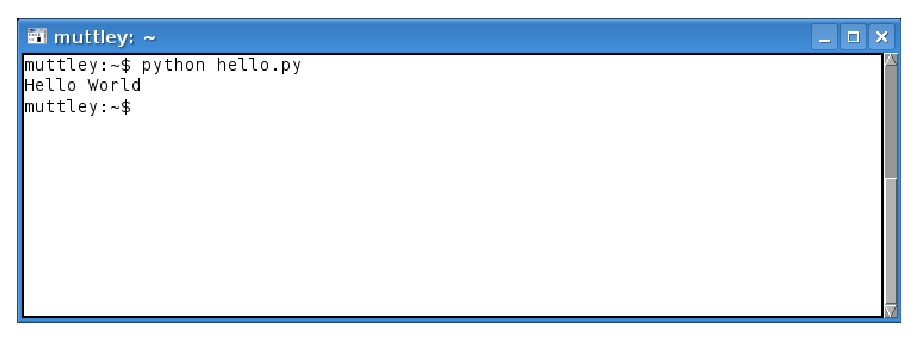
\includegraphics[width=75mm]{figure9.eps}
\end{center}
\caption{Running a python program from a text file on Linux.}\label{fig9}
\end{figure}
\end{LINUX}

Теперь ты видишь, что добрые люди, создавшие язык Python, спасли тебя от необходимости печатать одно и тоже снова и снова и снова и снова.  Как они делали в далеких 80'х. Нет, я серьёзно---они так делали.  Пойди спроси у своего папы, был ли у него когда-нибудь, когда он был по моложе, компьютер ZX81.\\

\noindent
Если был, можешь показать на него пальцем и посмеяться.\\

\noindent
Поверь мне.  Ты не поймешь этого.  Но он сообразит, о чём ты.\footnote{Синклер ZX81, выпущенный в 1980'х годах был одним из доступных домашних компьютеров.  Многие мальчишки и девчонки просто сходили с ума, перепечатывая исходные коды программ и игр из популярных в то время журналов по ZX81---только для того, чтобы после нескольких часов набивания текста обнаружить, эти бесполезные программы никогда не работали.}

\noindent
\emph{Так что будь готов быстренько убежать.}

\subsection*{\color{BrickRed}Заканчивая вступление}

Добро пожаловать в прекрасный мир Программирования.  Мы начали с самой простой программы ``Привет Мир''---все начинают с неё, когда учатся программировать.
В следующей главе мы будем делать более полезные вещи и посмотрим, как создаются программы.

\newpage
% ch2.tex
% This work is licensed under the Creative Commons Attribution-Noncommercial-Share Alike 3.0 New Zealand License.
% To view a copy of this license, visit http://creativecommons.org/licenses/by-nc-sa/3.0/nz
% or send a letter to Creative Commons, 171 Second Street, Suite 300, San Francisco, California, 94105, USA.


\chapter{8 умножить на 3.57 равно$\ldots$}\label{ch:8multipliedby3.57}

Сколько будет 8 умножить на 3.57?  Ты бы использовал калькулятор, верно? Или может ты исключительно умен, что можешь умножать дроби в уме---хотя, это не важно. Ты можешь делать то же самое в используя консоль Python. Снова запусти консоль (смотри Главу~\ref{ch:notallsnakeswillsquishyou} для подробностей, если ты пропустил её по какой-то странной причине) и когда ты увидишь приглашение, напечатай 8$*$3.57 и нажми клавишу Enter:

\begin{listing}
\begin{verbatim}
Python 3.0 (r30:67503, Dec  6 2008, 23:22:48) 
Type "help", "copyright", "credits" or "license" for more information.
>>> 8 * 3.57
28.559999999999999
\end{verbatim}
\end{listing}

Звездочка (*) используется для умножения\index{multiplication}, вместо обычного символа (\textsf{X}) который ты используешь в школе (применение символа звездочки необходимо, иначе компьютеру было бы не понять, используешь ли ты обычную букву \emph{x} или знак умножения \textsf{X} ?).  Как на счёт более полезного уравнения?

Предположим, что раз в неделю ты делаешь домашние задания, за которые получаешь \$5 карманных денег, и еще ты разносишь газеты 5 раз в неделю и получаешь за это по \$30---сколько бы денег ты заработал за год?

\begin{figure}[t]
\begin{center}
\fbox{\colorbox{PaleBlue}{\parbox{.75\linewidth} {
\subsection*{Python сломался!?!?}

Если ты сейчас возьмешь калькулятор и посчитаешь 8x3.57 ответ на экране будет:\\

\textsf{
28.56\\
}

\noindent
Почему ответ Python отличается?  Он сломан?\\

\noindent
На самом деле, нет. Причина в том, как компьютер иначе обрабатывает числа с плавающей точкой\index{floating point}(числа с целой и дробной частью). Это сложная и, порой, сбивающая с толку проблема для новичков, так что проще просто запомнить, что при работе с дробями (т.е. с числами с точкой) \emph{иногда} результат будет не совсем таким, как ты ожидаешь. Это так же действует для умножения, деления, сложения и вычитания. 
}}}
\end{center}
\end{figure}

Если бы мы писали это на бумаге, мы бы написали что-то подобное:
\begin{verbatim}
(5 + 30) x 52
\end{verbatim}

Что означает \$5 + \$30 умножить на 52 недели в году.  \begin{samepage}Конечно, мы умны, и знаем, что 5 + 30 равно 35, так что формула на самом деле такая:

\begin{verbatim}
35 x 52
\end{verbatim}
\end{samepage}

Которая достаточно проста, чтобы посчитать её на калькуляторе или на бумаге.  Но мы можем посчитать все это и в консоли:

\begin{listing}
\begin{verbatim}
>>> (5 + 30) * 52
1820
>>> 35 * 52
1820
\end{verbatim}
\end{listing}

А что, если бы ты тратил \$10 каждую неделю? Сколько бы у тебя осталось к концу года? Мы могли бы записать эту формулу на бумаге несколькими разными способами, но давай просто наберем её в консоли:

\begin{listing}
\begin{verbatim}
>>> (5 + 30 - 10) * 52
1300
\end{verbatim}
\end{listing}

Это означает \$5 и \$30 минус \$10 умноженные на 52 недель в году.  И у тебя остаётся \$1300 к концу года. Хорошо, пока что это всё не выглядит так уж полезно.  Мы можем сделать всё это с помощью калькулятора.  Но мы вернемся к этому позднее и покажем, как сделать пример значительно полезнее.

Ты можешь делать умножение\index{multiplication} и сложение\index{addition} (очевидно), и вычитание\index{subtraction} и деление\index{division} в консоли Python, вместе с набором других математических операций, которые мы пока не будем тут рассматривать. Пока что основные математические символы в Python (на самом деле, они называются операторы\index{operators}) следующие:

\begin{center}
\begin{tabular}{|c|c|}
\hline
+ & Сложение \\
\hline
- & Вычитание \\
\hline
* & Умножение \\
\hline
/ & Деление \\
\hline
\end{tabular}
\end{center}

Причина, по которой косая черта (/) используется для деления в том, что было бы достаточно трудно нарисовать линию деления (к тому же, они не потрудились добавить знак деления $\div$ на клавиатуру компьютера), как ты, вероятно, делаешь с письменными формулами. Например, если у тебя было 100 яиц и 20 ящиков, ты бы мог узнать, по сколько яиц попало бы в каждый ящик, поэтому ты бы написал следующую формулу, разделив 100 на 20:
\begin{displaymath}
\frac{100}{20}
\end{displaymath}

Или, если ты знаком с делением в столбик, то мог бы записать это так:

\begin{displaymath}
\longdiv{100}{20}
\end{displaymath}

Или даже так:

\begin{displaymath}
100 \div 20
\end{displaymath}

Однако, на языке Python ты бы просто набрал ``100 / 20''.

\emph{Что значительно проще, я думаю.  Но, когда я - книга---что я могу знать?}

\section{Использование скобок и ``Порядок Операций''}\index{order of operations}

В языке программирования мы используем скобки для управления так называемым ``Порядком Операций''.  Операцией называется факт использования оператора (одного из тех символов в таблице выше). Существуют и другие операторы кроме этих символов, но для нашего простого списка (сложение, вычитание, умножение и деление) достаточно знать, что умножение и деление имеют более высокий приоритет чем сложение и вычитание.  Это означает, что сначала ты выполняешь все умножения или деления в выражении, а потом сложения и вычитания.  В следующем выражении все операции являются сложениями (+), поэтому числа складываются по порядку:

\begin{listing}
\begin{verbatim}
>>> print(5 + 30 + 20)
55
\end{verbatim}
\end{listing}

\noindent
Similarly, in this equation, there are only addition and subtraction operators, so again Python considers each number in the order it appears:

\begin{listing}
\begin{verbatim}
>>> print(5 + 30 - 20)
15
\end{verbatim}
\end{listing}

\noindent
But in the following equation, there is a multiplication operator, so the numbers 30 and 20 are considered first.  The equation is another way of saying, ``multiply 30 by 20, then add 5 to the result'' (multiplication first, because it has a higher order than addition):

\begin{listing}
\begin{verbatim}
>>> print(5 + 30 * 20)
605
\end{verbatim}
\end{listing}

\noindent
So what happens when we add brackets?  The following equation shows the result:

\begin{listing}
\begin{verbatim}
>>> print((5 + 30) * 20)
700
\end{verbatim}
\end{listing}

\noindent
Why is the number different?  Because brackets control the order of operations.  With brackets, Python knows to calculate using the operators in the brackets first, then do the operators outside.  So that equation is another way of saying, ``add 5 and 30, then multiply the result by 20''.
The use of brackets can become more complicated.  There can be brackets inside brackets:

\begin{listing}
\begin{verbatim}
>>> print(((5 + 30) * 20) / 10)
70
\end{verbatim}
\end{listing}

\noindent
In this case, Python evaluates the \textbf{inner} most brackets first, then the outer brackets, and then the other operator.  So this equation is a way of saying, ``add 5 and 30, then multiply the result by 20, finally divide that result by 10''.  The result without brackets is again slightly different:

\begin{listing}
\begin{verbatim}
>>> 5 + 30 * 20 / 10
65
\end{verbatim}
\end{listing}

In this case 30 is multiplied by 20 first, then the result is divided by 10, finally 5 is added to the final result.

\emph{Remember that multiplication and division always go before addition and subtraction, unless brackets are used to control the order of operations.}

\section{There's nothing so fickle as a variable}\index{variable}

A `variable' is a programming term used to describe a place to store things.  The `things' can be numbers, or text, or lists of numbers and text---and all sorts of other items too numerous to go into here.  For the moment, let's just think of a variable as something a bit like a mailbox.

\begin{center}
\includegraphics*[width=76mm]{girlbubble.eps}
\end{center}

You can put things (such as a letter or a package) in a mailbox, just as you can put things (numbers, text, lists of numbers and text, etc, etc, etc) in a variable.  This mailbox idea is the way many programming languages work.  But not all.

In Python, variables are slightly different.  Rather than being a mailbox with things in it, a variable is more like a label which is stuck on the outside of the mailbox.  We can pull that label off and stick it on something else, or even tie the label (perhaps with a piece of string) to more than one thing. We create a variable by giving it a name, using an equals sign (=), then telling Python what we want that name to point to.  For example:

\begin{listing}
\begin{verbatim}
>>> fred = 100
\end{verbatim}
\end{listing}

We've just created a variable called `fred' and said that it points to the number 100.  It's a bit like telling Python to remember that number because we want to use it later.  To find out what a variable is pointing at, we can just type `print' in the console, followed by the variable name, and hit the Enter key.  For example:

\begin{listing}
\begin{verbatim}
>>> fred = 100
>>> print(fred)
100
\end{verbatim}
\end{listing}

We can also tell Python we want the variable \code{fred} to point at something else:

\begin{listing}
\begin{verbatim}
>>> fred = 200
>>> print(fred)
200
\end{verbatim}
\end{listing}

\noindent
On the first line we say we now want fred to point at the number 200.  Then, in the second line, we ask what fred is pointing at just to prove it changed. We can also point more than one name at the same item:

\begin{listing}
\begin{verbatim}
>>> fred = 200
>>> john = fred
>>> print(john)
200
\end{verbatim}
\end{listing}

In the code above, we're saying that we want the name (or label) \code{john} to point at the same thing \code{fred} is pointing to.
Of course, `fred' isn't a very useful name for a variable.  It doesn't tell us anything about what it's used for.  A mailbox is easy---you use a mailbox for mail.  But a variable can have a number of different uses, and can point at a whole bunch of different things, so we usually want something more informative as its name.
\par
Suppose you started up the Python console, typed `fred = 200', then went away---spent 10 years climbing Mount Everest, crossing the Sahara desert, bungy-jumping off a bridge in New Zealand, and finally, sailing down the Amazon river---when you came back to your computer, would you remember what that number 200 meant (and what it was for)?

\noindent
\emph{I don't think I would.}

\noindent
I just made it up now, and I have no idea what `fred = 200' means (other than a \emph{name} pointing at the number \emph{200}).  So after 10 years, you'll have absolutely no chance of remembering.
\par
Aha!  But, what if we called our variable: \emph{number\_of\_students}.

\begin{listing}
\begin{verbatim}
>>> number_of_students = 200
\end{verbatim}
\end{listing}

We can do that because variable names can be made up of letters, numbers and (\_) underscores---although they cannot start with a number.  If you come back after 10 years, `number\_of\_students' still makes sense.  You can type:

\begin{listing}
\begin{verbatim}
>>> print(number_of_students)
200
\end{verbatim}
\end{listing}

\noindent
And you'll immediately know that we're talking about 200 students.  It's not always important to come up with meaningful names for variables.  You can use anything from single letters (such as `a') to large sentences; and sometimes, if you're doing something quick, a simple and short variable name is just as useful.  It depends very much upon whether you want to be able to look at that variable name later and figure out what on earth you were thinking at the time you typed it in.

\begin{listing}
\begin{verbatim}
this_is_also_a_valid_variable_name_but_perhaps_not_very_useful
\end{verbatim}
\end{listing}

\section{Using Variable}\index{Variables}

Now we know how to create a variable, how do we use it?  Remember that equation we came up with earlier?  The one to work out how much money you'd have left at the end of the year, if you earned \$5 a week doing chores, \$30 a week on a paper round, and spent \$10 per week.  So far we have:

\begin{listing}
\begin{verbatim}
>>> print((5 + 30 - 10) * 52)
1300
\end{verbatim}
\end{listing}

\noindent
What if we turn the first 3 numbers into variables?  Try typing the following:

\begin{listing}
\begin{verbatim}
>>> chores = 5
>>> paper_round = 30
>>> spending = 10
\end{verbatim}
\end{listing}

\noindent
We've just created variables named `chores', `paper\_round' and `spending'.  We can then re-type the equation to get:

\begin{listing}
\begin{verbatim}
>>> print((chores + paper_round - spending) * 52)
1300
\end{verbatim}
\end{listing}

Which gives the exact same answer.  What if you get \$2 more per week, for doing extra chores.  Change the `chores' variable to 7, then hit the up-arrow key ($\uparrow$) on your keyboard a couple of times, until the equation re-appears, and hit the Enter key:

\begin{listing}
\begin{verbatim}
>>> chores = 7
>>> print((chores + paper_round - spending) * 52)
1404
\end{verbatim}
\end{listing}

That's a lot less typing to find out that you now end up with \$1404 at the end of the year.  You can try changing the other variables, then hit the up-arrow to perform the calculation again, and see what effect it has.

\begin{listing}
\begin{verbatim}
If you spend twice as much money per week:
>>> spending = 20
>>> print((chores + paper_round - spending) * 52)
884
\end{verbatim}
\end{listing}

You're only left with \$884 savings at the end of the year. This is still only slightly useful.  We haven't hit really useful yet.  But for the moment, it's enough to understand that variables are used to store things.

\noindent
\emph{Think of a mailbox with a label on it!}

\section{A Piece of String?}\index{strings}

If you're paying attention, and not just skimming through looking for the good bits, you might remember I mentioned that variables can be used for all sorts of things---not just numbers. In programming, most of the time we call text a `string'. Which might seem a bit weird; but if you think that text is just `stringing together' (or joining together) a bunch of letters, perhaps it might make a little more sense.

\noindent
\emph{Then again, perhaps it doesn't.}

In which case, all you need to know, is that a string is just a bunch of letters and numbers and other symbols put together in some meaningful way. All the letters, and numbers, and symbols in this book could make up a string.  Your name could be a string.  So could your home address.  The first Python program we created in Chapter \ref{ch:notallsnakeswillsquishyou}, used a string: `Hello World'.
\par
In Python, we create a string by putting quotes around the text.  So we can take our useless \code{fred} variable, and put a string inside it like this:

\begin{listing}
\begin{verbatim}
>>> fred = "this is a string"
\end{verbatim}
\end{listing}

\noindent
And we can see what's inside the \code{fred} variable, by typing \code{print(fred)}:

\begin{listing}
\begin{verbatim}
>>> print(fred)
this is a string
\end{verbatim}
\end{listing}

\noindent
We can also use single-quotes to create a string:

\begin{listing}
\begin{verbatim}
>>> fred = 'this is yet another string'
>>> print(fred)
this is yet another string
\end{verbatim}
\end{listing}

However, if you try to type more than one line of text for your string using a single quote (') or double quote ("), you'll get an error message in the console. For example, type the following line and hit Enter, and you'll get a fairly scary error message similar to the following:

\begin{listing}
\begin{verbatim}
>>> fred = "this is two
  File "<stdin>", line 1
    fred = "this is two
                      ^
SyntaxError: EOL while scanning string literal
\end{verbatim}
\end{listing}

\index{multi-line string}We'll talk more about errors later, but for the moment, if you want more than one line of text, you can use 3 single quotes:

\begin{listing}
\begin{verbatim}
>>> fred = '''this is two
... lines of text in a single string'''
\end{verbatim}
\end{listing}

\noindent
Print out the contents to see if it worked:

\begin{listing}
\begin{verbatim}
>>> print(fred)
this is two
lines of text in a single string
\end{verbatim}
\end{listing}

By the way, you'll see those 3 dots (...) quite a few times when you're typing something that continues onto another line (like a multi line string).  In fact, you'll see it a lot more as we continue.

\section{Tricks with Strings}\label{trickswithstrings}

Here's an interesting question:  what's 10 * 5 (10 times 5)?  The answer is, of course, 50.

\noindent
\emph{All right, that's not an interesting question at all.}

But what is 10 * 'a' (10 times the letter a)?  It might seem like a nonsensical question, but here's the answer from the World of Python:

\begin{listing}
\begin{verbatim}
>>> print(10 * 'a')
aaaaaaaaaa
\end{verbatim}
\end{listing}

This works with more than just single character strings:

\begin{listing}
\begin{verbatim}
>>> print(20 * 'abcd')
abcdabcdabcdabcdabcdabcdabcdabcdabcdabcdabcdabcdabcdabcdabcdabcdabcdabcdabcdabcd
\end{verbatim}
\end{listing}

Another trick with a string, is embedding values.  You can do this by using \%s, which is like a marker (or a placeholder) for a value you want to include in a string.  It's easier to explain with an example:

\begin{listing}
\begin{verbatim}
>>> mytext = 'I am %s years old'
>>> print(mytext % 12)
I am 12 years old
\end{verbatim}
\end{listing}

In the first line, the variable mytext is created with a string containing some words and a placeholder (\%s).  The \%s is a little beacon saying ``replace me with something'' to the Python console.  So on the next line, when we call \code{print(mytext)}, we use the \% symbol, to tell Python to replace the marker with the number 12. We can reuse that string and pass in different values:

\begin{listing}
\begin{verbatim}
>>> mytext = 'Hello %s, how are you today?'
>>> name1 = 'Joe'
>>> name2 = 'Jane'
>>> print(mytext % name1)
Hello Joe, how are you today?
>>> print(mytext % name2)
Hello Jane, how are you today?
\end{verbatim}
\end{listing}

In the above example, 3 variables (mytext, name1 and name2) are created---the first includes the string with the marker.  Then we can print the variable `mytext', and again use the \% operator to pass in variables `name1' and `name2'.  You can use more than one placeholder:

\begin{listing}
\begin{verbatim}
>>> mytext = 'Hello %s and %s, how are you today?'
>>> print(mytext % (name1, name2))
Hello Joe and Jane, how are you today?
\end{verbatim}
\end{listing}

When using more than one marker, you need to wrap the replacement values with brackets---so (name1, name2) is the proper way to pass 2 variables. A set of values surrounded by brackets (the round ones, not the square ones) is called a \emph{tuple}, and is a little bit like a list, which we'll talk about next.

\section{Not quite a shopping list}\index{lists}

Eggs, milk, cheese, celery, peanut butter, and baking soda.  Which is not quite a full shopping list, but good enough for our purposes. If you wanted to store this in a variable you could create a string:

\begin{listing}
\begin{verbatim}
>>> shopping_list = 'eggs, milk, cheese, celery, peanut butter, baking soda'
>>> print(shopping_list)
eggs, milk, cheese, celery, peanut butter, baking soda
\end{verbatim}
\end{listing}

Another way would be to create a `list', which is a special kind of object in Python:

\begin{listing}
\begin{verbatim}
>>> shopping_list = [ 'eggs', 'milk', 'cheese', 'celery', 'peanut butter', 
... 'baking soda' ]
>>> print(shopping_list)
['eggs', 'milk', 'cheese', 'celery', 'peanut butter', 'baking soda']
\end{verbatim}
\end{listing}

This is more typing, but it's also more useful.  We could print the 3rd item in the list by using its position (called its index position), inside square brackets []:

\begin{listing}
\begin{verbatim}
>>> print(shopping_list[2])
cheese
\end{verbatim}
\end{listing}

Lists start at index position 0---so the first item in a list is 0, the second is 1, the third is 2.  That doesn't make a lot of sense to most people, but it does to programmers.  Pretty soon, when you walk up some stairs you'll start counting with zero rather than one.  That will really confuse your little brother or sister.
\par
We can show all the items from the 3rd item up to the 5th in the list, by using a colon inside the square brackets:

\begin{listing}
\begin{verbatim}
>>> print(shopping_list[2:5])
['cheese', 'celery', 'peanut butter']
\end{verbatim}
\end{listing}

[2:5] is the same as saying that we are interested in items from index position 2 up to (but not including) index position 5.  And, of course, because we start counting with 0, the 3rd item in the list is actually number 2, and the 5th item is actually number 4. Lists can be used to store all sorts of items.  They can store numbers:

\begin{listing}
\begin{verbatim}
>>> mylist = [ 1, 2, 5, 10, 20 ]
\end{verbatim}
\end{listing}

\noindent
And strings:

\begin{listing}
\begin{verbatim}
>>> mylist = [ 'a', 'bbb', 'ccccccc', 'ddddddddd' ]
\end{verbatim}
\end{listing}

\noindent
And mixtures of numbers and strings:

\begin{listing}
\begin{verbatim}
>>> mylist = [1, 2, 'a', 'bbb']
>>> print(mylist)
[1, 2, 'a', 'bbb']
\end{verbatim}
\end{listing}

\noindent
And even lists of lists:

\begin{listing}
\begin{verbatim}
>>> list1 = [ 'a', 'b', 'c' ]
>>> list2 = [ 1, 2, 3 ]
>>> mylist = [ list1, list2 ]
>>> print(mylist)
[['a', 'b', 'c'], [1, 2, 3]]
\end{verbatim}
\end{listing}

In the above example, a variable called `list1' is created with 3 letters, `list2' is created with a 3 numbers, and `mylist' is created using list1 and list2. Things can get rather confusing, rather quickly, if you start creating lists of lists of lists of lists$\ldots$ but luckily there's not usually much need for making things that complicated in Python. Still it is handy to know that you can store all sorts of items in a Python list.

\noindent
\emph{And not just your shopping.}

\subsection*{\color{BrickRed}Replacing items}\index{lists!replacing}

We can replace an item in the list, by setting its value in a similar way to setting the value of a normal variable. For example, we could change celery to lettuce by setting the value in index position 3:

\begin{listing}
\begin{verbatim}
>>> shopping_list[3] = 'lettuce'
>>> print(shopping_list)
['eggs', 'milk', 'cheese', 'lettuce', 'peanut butter', 'baking soda']
\end{verbatim}
\end{listing}

\subsection*{\color{BrickRed}Adding more items...}\index{lists!appending}

We can add items to a list by using a method called `append'.  A method is an action or command that tells Python that we want to do something.  We'll talk more about methods later, but for the moment, to add an item to our shopping list, we can do the following:

\begin{listing}
\begin{verbatim}
>>> shopping_list.append('chocolate bar')
>>> print(shopping_list)
['eggs', 'milk', 'cheese', 'lettuce', 'peanut butter', 'baking soda', 
'chocolate bar']
\end{verbatim}
\end{listing}

Which, if nothing else, is certainly an improved shopping list.

\subsection*{\color{BrickRed}$\ldots$and removing items}\index{lists!removing}

We can remove items from a list by using the command `del' (short for delete).  For example, to remove the 6th item in the list (baking soda):

\begin{listing}
\begin{verbatim}
>>> del shopping_list[5]
>>> print(shopping_list)
['eggs', 'milk', 'cheese', 'lettuce', 'peanut butter', 'chocolate bar']
\end{verbatim}
\end{listing}

Remember that positions start at zero, so shopping\_list[5] actually refers to the 6th item.

\subsection*{\color{BrickRed}2 lists are better than 1}\index{lists!joining}

We can join lists together by adding them, as if we were adding two numbers:

\begin{listing}
\begin{verbatim}
>>> list1 = [ 1, 2, 3 ]
>>> list2 = [ 4, 5, 6 ]
>>> print(list1 + list2)
[1, 2, 3, 4, 5, 6]
\end{verbatim}
\end{listing}

\noindent
We can also add the two lists and set the result to another variable:

\begin{listing}
\begin{verbatim}
>>> list1 = [ 1, 2, 3 ]
>>> list2 = [ 4, 5, 6 ]
>>> list3 = list1 + list2
>>> print(list3)
[1, 2, 3, 4, 5, 6]
\end{verbatim}
\end{listing}

\noindent
And you can multiply a list in the same way we multiplied a string:

\begin{listing}
\begin{verbatim}
>>> list1 = [ 1, 2 ]
>>> print(list1 * 5)
[1, 2, 1, 2, 1, 2, 1, 2, 1, 2]
\end{verbatim}
\end{listing}

\noindent
In the above example, multiplying list1 by five is another way of saying ``repeat list1 five times''. However, division (/) and subtraction (-) don't make sense when working with lists, so you'll get errors when trying the following examples:

\begin{listing}
\begin{verbatim}
>>> list1 / 20
Traceback (most recent call last):
  File "<stdin>", line 1, in <module>
TypeError: unsupported operand type(s) for /: 'list' and 'int'
\end{verbatim}
\end{listing}

\noindent
or:

\begin{listing}
\begin{verbatim}
>>> list1 - 20
Traceback (most recent call last):
  File "<stdin>", line 1, in <module>
TypeError: unsupported operand type(s) for -: 'type' and 'int'
\end{verbatim}
\end{listing}

\noindent
You'll get a rather nasty error message.

\section{Tuples and Lists}\label{tuplesandlists}\index{tuples}

A tuple (mentioned earlier) is a little bit like a list, but rather than using square brackets, you use round brackets---e.g. `(' and `)'.  You can use tuples in a similar way to a list:

\begin{listing}
\begin{verbatim}
>>> t = (1, 2, 3)
>>> print(t[1])
2
\end{verbatim}
\end{listing}

The main difference is that, unlike lists, tuples can't change, once you've created them.  So if you try to replace a value like we did earlier with the list, you'll get another error message:

\begin{listing}
\begin{verbatim}
>>> t[0] = 4
Traceback (most recent call last):
  File "<stdin>", line 1, in ?
TypeError: 'tuple' object does not support item assignment
\end{verbatim}
\end{listing}

That doesn't mean you can't change the variable containing the tuple to something else.  For example, this code will work fine:

\begin{listing}
\begin{verbatim}
>>> myvar = (1, 2, 3)
>>> myvar = [ 'a', 'list', 'of', 'strings' ]
\end{verbatim}
\end{listing}

First we create the variable \code{myvar} pointing to a tuple of 3 numbers.  Then we change \code{myvar} to point at a list of strings. This might be a bit confusing at first.  But think of it like lockers in a school.  Each locker has a name tag on it. You put something in the locker, close the door, lock it, then throw away the key.  You then peel the name tag off, wander over to another empty locker, and stick something else in that (but this time you keep the key).  A tuple is like the locked locker.  You can't change what's inside it.  But you can take the label off and stick it on an unlocked locker, and then put stuff inside that locker and take stuff out---that's the list.

\section{Things to try}

\emph{In this chapter we saw how to calculate simple mathematical equations using the Python console.  We also saw how brackets can change the result of an equation, by controlling the order that operators are used.  We found out how to tell Python to remember values for later use---using variables---plus how Python uses `strings' for storing text, and lists and tuples, for handling more than one item.}
\par

\subsection*{Exercise 1}
Make a list of your favourite toys and name it \code{toys}.  Make a list of your favourite foods and name it \code{foods}.  Join these two lists and name the result \code{favourites}.  Finally print the variable \code{favourites}.

\subsection*{Exercise 2}
If you have 3 boxes containing 25 chocolates, and 10 bags containing 32 sweets, how many sweets and chocolates do you have in total?  (Note: you can do this with one equation with the Python console)

\subsection*{Exercise 3}
Create variables for your first and last name. Now create a string and use placeholders to add your name.


\newpage
\include{ch3}
\include{ch4}
\include{ch5}
\include{ch6}
\include{ch7}
\include{ch8}
\include{ch9}
\include{ch10}

\appendix
\include{appendixa}
\include{appendixb}
\include{appendixc}
\include{appendixd}

\printindex

\end{document}
